\begin{center}
\subsubsection*{Abstract}
\end{center}
\item{Are business analysis techniques. Both techniques are useful to improve organizational performance. But their applications differ. Both can be used together with the key performance indicators to monitor and improve the performance of the organization. We will understand both the technique and the detail.
\\
\textbf{}
\\
The Balanced Scorecard (CMI Spanish Acronym) and the Canvas model can be linked as complementary tools for entrepreneurs. The first develops goals and operational measures in four main perspectives for the purpose of achieving the mission and strategy. The second suggest a (re-) evolution in generating business models, establishing nine sections that reflect their logic. In the article a working model is developed that, based on the need for a CMI it relates its design to the information previously collected in the Canvas model, pointing their mutual necessity.}

\begin{center}
\subsubsection*{Resumén}
\end{center}
\item{Son técnicas de análisis empresarial . Ambas técnicas son útiles para mejorar el desempeño organizacional. Pero sus aplicaciones difieren. Ambos se pueden usar junto con los indicadores clave de rendimiento para monitorear y mejorar el rendimiento de la organización. Vamos a entender tanto la técnica en detalle.
\\
\textbf{}
\\
El Cuadro de Mando Integral (BSC) y el modelo Canvas pueden enlazarse como herramientas complementarias para los emprendedores. La primera desarrolla objetivos y medidas operativas en cuatro perspectivas principales para alcanzar la misión y estrategia. La segunda ha supuesto una (re-)evolución en la generación de modelos de negocio, estableciendo nueve apartados que reflejan su lógica. En el artículo se desarrolla un modelo de trabajo que, partiendo de la necesidad de disponer de un BSC, relaciona su diseño con la información recogida previamente en el modelo Canvas, señalando su mutua necesidad.}

\newpage

\begin{center}
    Trabajo Encargado N° 03 - BSC Y BMC
\end{center}

\section{Introducción}
\item{Esta metodología deriva de la gestión estratégica de empresas y presupone una elección de indicadores que no debe ser restringida al área económico – financiera. Así como no es posible comandar un avión controlando apenas la velocidad, los indicadores financieros no son suficientes para garantizar que una empresa se dirija en la dirección correcta. Por estos motivos, será necesario monitorear, junto a los indicadores económicos –financieros, el desempeño de mercado, los procesos internos, la innovación y la tecnología. De este modo, los resultados financieros serán fruto de la sumatoria de acciones generadas por personas a través del uso de las mejores tecnologías, vinculación a las mejores prácticas y los procesos internos de la organización, todo esto en armoníacon la Propuesta de Valor ofrecida al cliente. Esto proceso se denomina "crear valor através de activos intangibles"}

\begin{center}
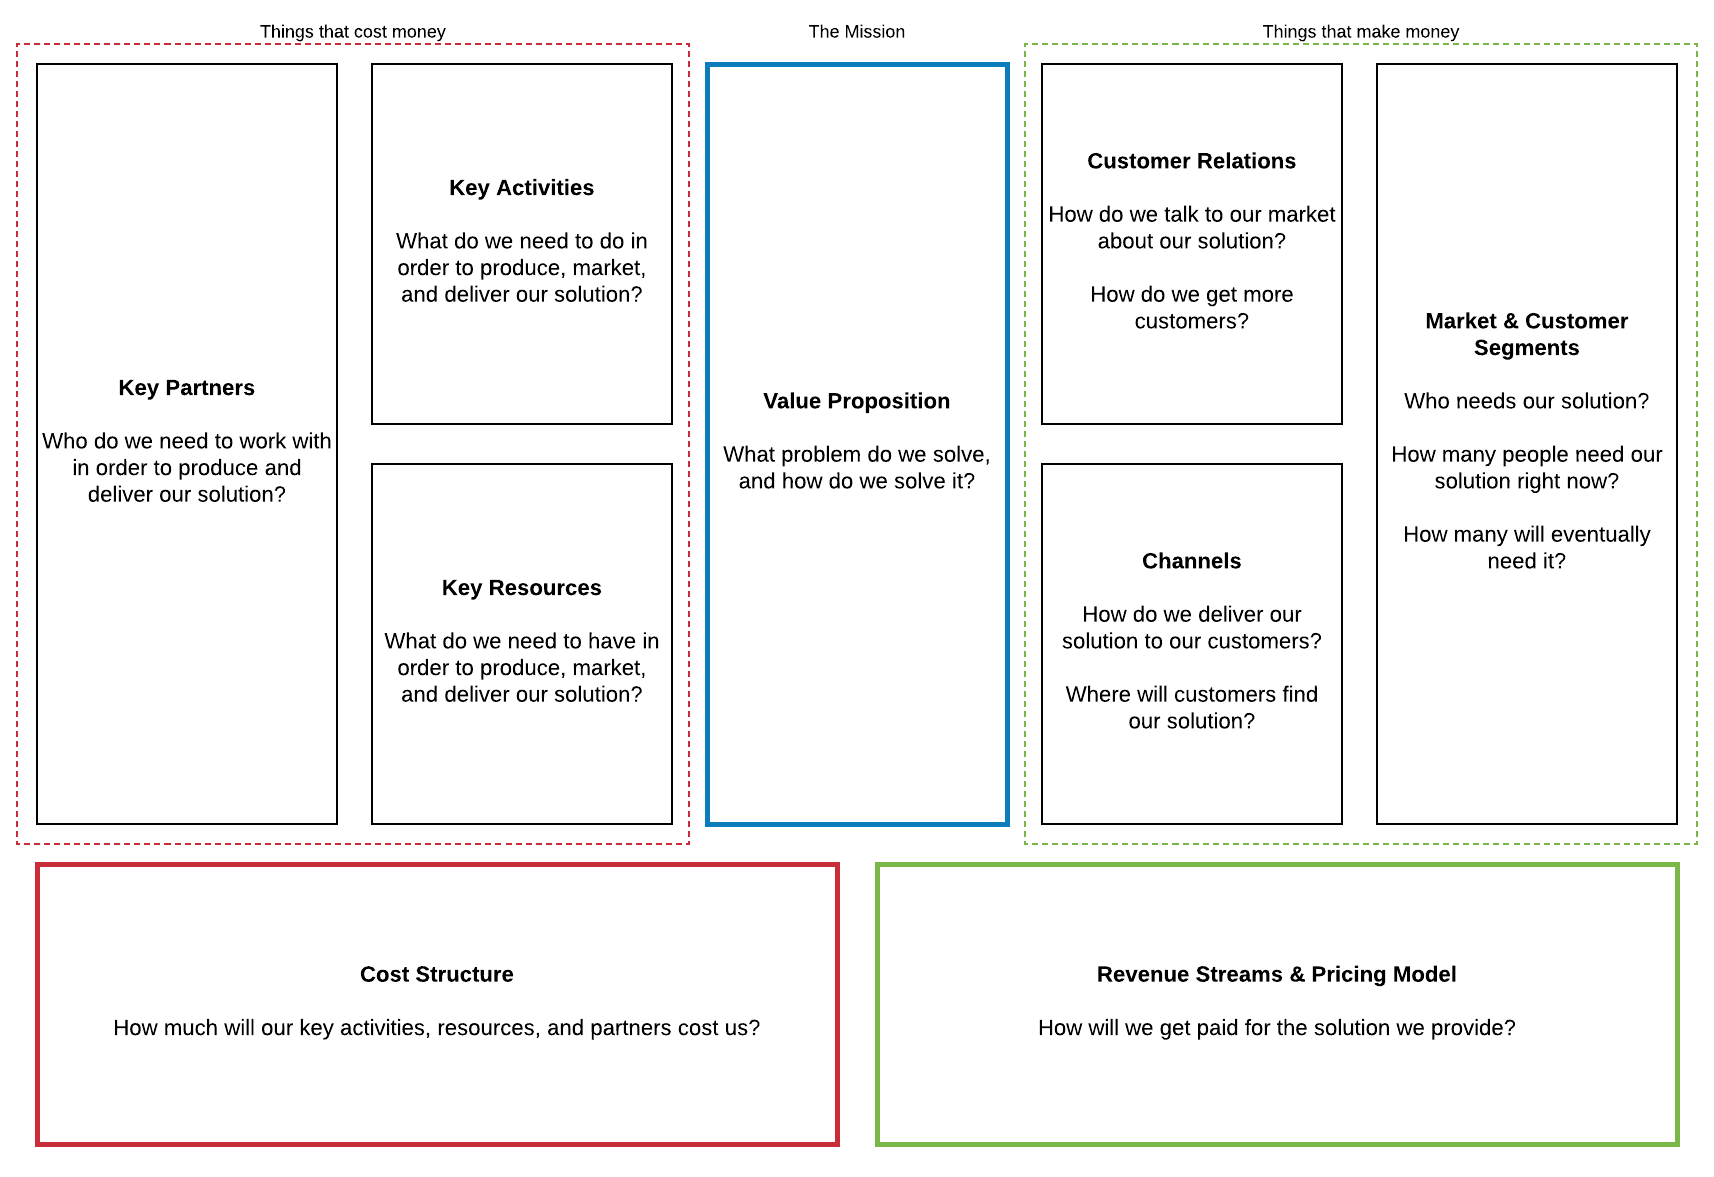
\includegraphics[width=10cm]{./Imagenes/img7}
\end{center}

\item{Balanced Scorecard ofrece una visión integrada y balanceada de la empresa y permite desarrollar la estrategia en forma clara. Esto se logra a través de objetivos estratégicos identificados en 4 perspectivas: financiera, clientes, procesos internos yaprendizaje e innovación. Cada una de las perspectivas se vincula con las demás mediante relaciones de causa y efecto. BSC promueve, además, el alineamiento de losobjetivos estratégicos con indicadores de desempeño, metas y planes de acción para hacer posible la generación de estrategias en forma integrada y garantizar que los esfuerzos de la organización se encuentren en línea con las mismas.}

\item{De acuerdo con el informe Global Entrepreneurship Monitor (GEM) del año 2012, a pesar de que en España la actividad emprendedora ha aumentado en los últimos años, son necesarios más esfuerzos para consolidar las nuevas empresas. Se reconoce ampliamente que su desarrollo y supervivencia no depende tanto de tener una buena idea de negocio sino de su adecuada ejecución y gestión. En este sentido, desde diferentes ámbitos se defiende que los emprendedores/as necesitan herramientas que les permitan desarrollar sus estrategias y les indiquen el grado de consecución de sus objetivos y actividades como medio de incrementar su probabilidad de supervivencia (\footnote{Davila & Oyon, 2009}).}

\item{En la literatura de dirección estratégica, el cuadro de mando integral (Balanced Scorecard, BSC de aquí en adelante) se considera como una de las herramientas más conocidas e importantes para la implementación de la estrategia (\footnote{Grant, 2006}). Su utilidad destaca en el momento de desarrollar objetivos operativos para la comunicación de la misión y estrategia de la empresa, así como en la medición del grado de consecución de éstas, proponiendo convertir la estrategia en un conjunto de medidas de actuación que permiten su traducción y gestión (\footnote{Kaplan y Norton, 1992}). De esta forma, un BSC ha de estar constituido por un conjunto limitado de medidas financieras y no financieras organizadas en cuatro principales perspectivas interrelacionadas entre sí (\footnote{Da Silva et al., 2013}), que describen la estrategia organizativa a través de relaciones causa-efecto entre los indicadores: (1) financiera, (2) cliente, (3) interna e (4) innovación y crecimiento.}

\section{Balanced Scorecard}

\item{El Balanced Scorecard, denominado BSC, es un marco para implementar y administrar la estrategia. Vincula una visión a objetivos estratégicos, medidas, metas e iniciativas. Equilibra las medidas financieras con las medidas de desempeño y los objetivos relacionados con todas las demás partes de la organización. Es una herramienta de gestión del rendimiento empresarial.}

\begin{center}
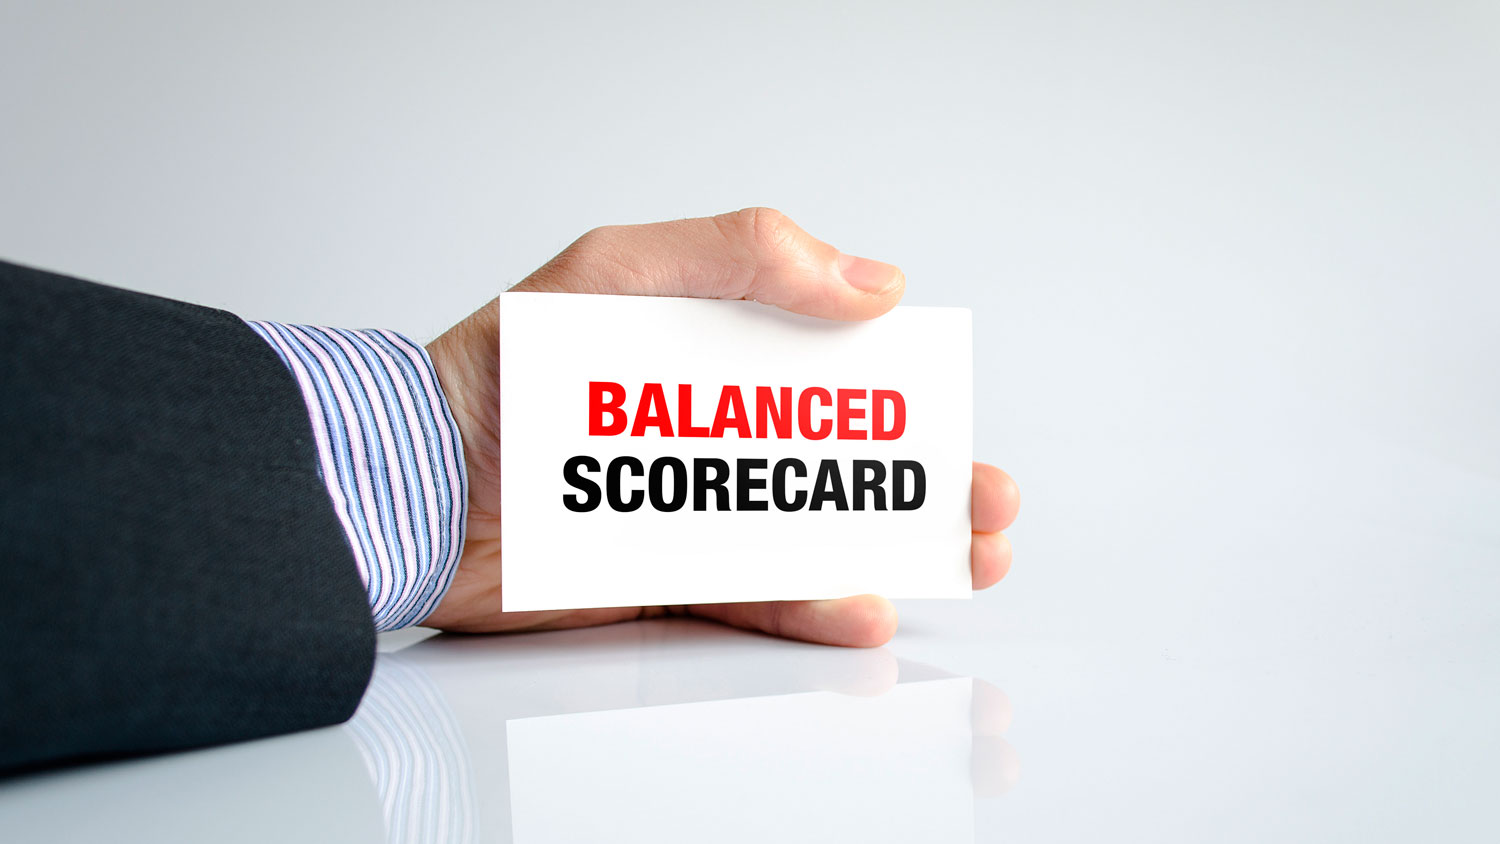
\includegraphics[width=15cm]{./Imagenes/img3}
\end{center}

\item{Fue publicado originalmente por el Dr. Robert Kaplan y el Dr. David Norton como un documento en 1992. Y luego formalmente como un libro en 1996. Tanto el documento como el libro llevaron a su éxito generalizado. Es interesante notar que aunque Kaplan y Norton publicaron el primer artículo, fueron referenciados de manera anómala en un trabajo de Art Schneiderman, quien se cree que es el creador del BSC.}

\begin{center}
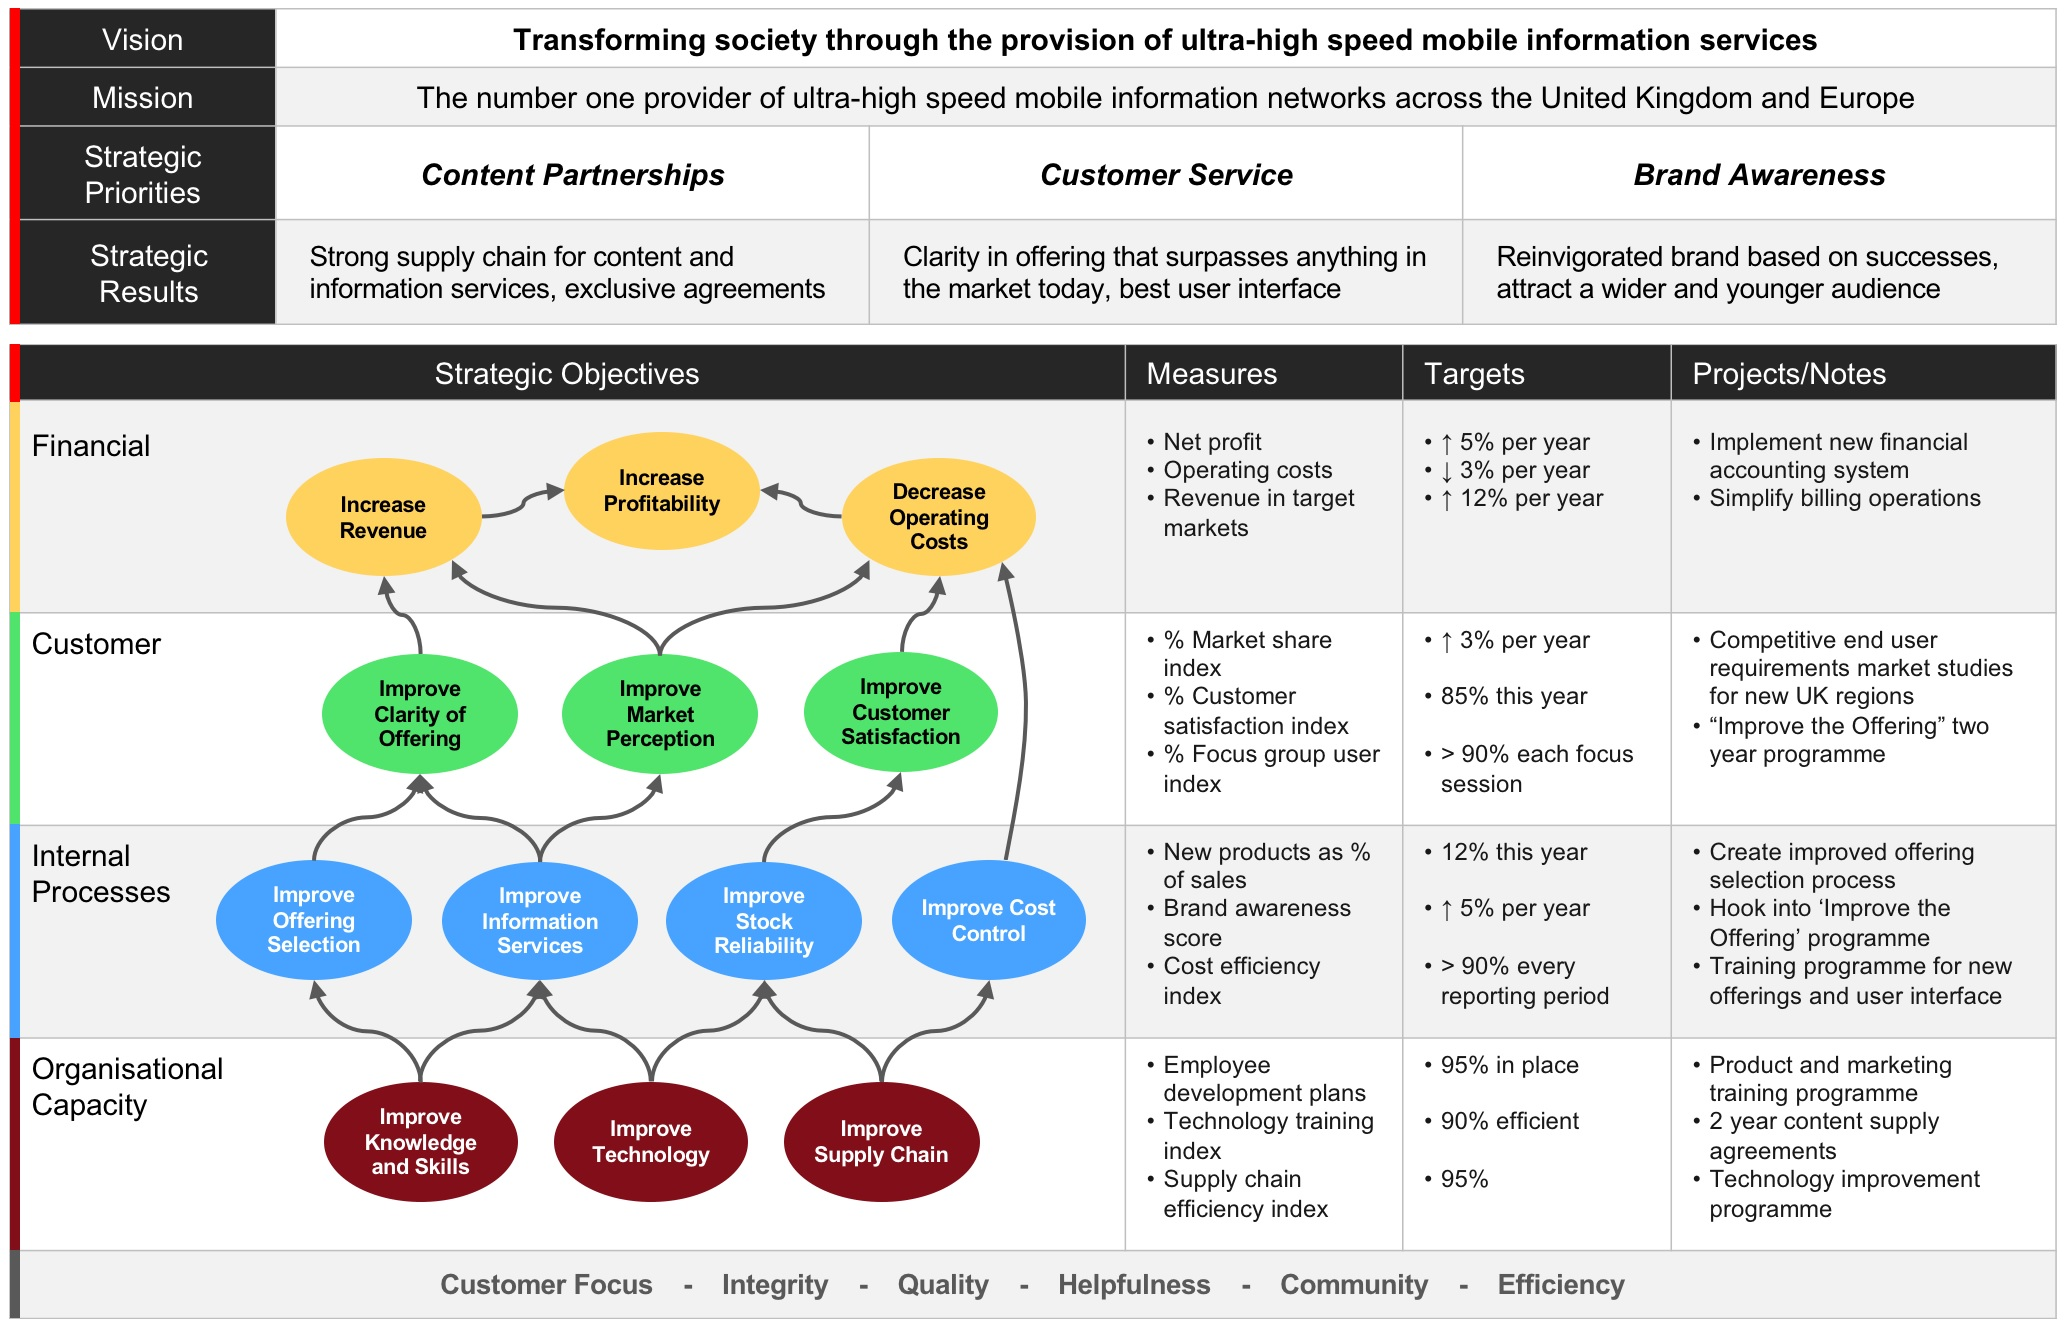
\includegraphics[width=17cm]{./Imagenes/img10}
\end{center}

\section*{Las cuatro perspectivas}
\item{A menudo surgen preguntas sobre las cuatro Perspectivas descritas en la metodología. ¿Por qué deberíamos considerar solo la capacidad financiera, de clientes, de procesos comerciales y organizativa? ¿Por qué no incluir salud y seguridad? La respuesta es, por supuesto, que nada nos detiene. Las cuatro perspectivas son simplemente un marco. Sin embargo, durante décadas de uso, ha quedado claro que funcionan.

Más importante aún, existe una relación causal entre las perspectivas. Trabajando de abajo hacia arriba: los cambios en la capacidad organizativa generarán cambios en los procesos comerciales que afectarán a los clientes y mejorarán los resultados financieros. La relación causal puede no estar garantizada si se agrega una nueva perspectiva. El resultado podría ser un cuadro de mando útil, pero no sería, por definición, un cuadro de mando equilibrado.}
\\
\item{En resumen, las cuatro perspectivas del cuadro de mando son:}
\textbf{}
\\
\item \textbf{Financial (Financiero):}
\item{Los objetivos financieros de alto nivel y las medidas financieras de la organización que ayudan a responder la pregunta: ¿Cómo miramos a nuestros accionistas? Los objetivos financieros suelen ser los más fáciles de definir y medir. Sin embargo, la creación de un objetivo financiero, por ejemplo, Mejorar el beneficio, rara vez proporciona una pista sobre cómo lograr el objetivo. Al vincular los objetivos de los niveles inferiores del modelo, comenzamos a ver exactamente dónde definir proyectos y realizar inversiones.}
\textbf{}
\\
\item \textbf{Customer (Cliente):}
\item{Objetivos y medidas que están directamente relacionados con los clientes de la organización, centrándose en la satisfacción del cliente. Para responder a la pregunta: ¿Cómo nos ven nuestros clientes? Siempre es importante dar un paso afuera y ver su empresa u organización desde el punto de vista de sus clientes. Debe comprender lo que quieren de usted, no necesariamente, qué puede hacer por ellos.}
\textbf{}
\\
\item \textbf{Internal Processes (Procesos internos):}
\item{Objetivos y medidas que determinan qué tan bien está funcionando el negocio y si los productos o servicios se ajustan a lo que requieren los clientes, en otras palabras, ¿en qué deberíamos ser mejores? Algunos de los artículos de mayor costo pueden reducirse mediante la racionalización de los procesos internos. Esta es también la mejor área para enfocarse en ideas nuevas y creativas.}
\textbf{}
\\
\item \textbf{Organisational Capacity (Capacidad Organizacional):}
\item{Objetivos y medidas sobre el desempeño de nuestra gente, sus habilidades, capacitación, cultura empresarial, liderazgo y base de conocimiento. Esta área también incluye infraestructura y tecnología. La capacidad organizativa tiende a ser el área donde se realiza la mayor parte de la inversión. Responde a la pregunta: ¿Cómo podemos mejorar y crear valor?
\\
\textbf{}
\\
El valor real del enfoque de Perspectiva es que proporciona un marco para describir una estrategia comercial. Se centra en objetivos y medidas que nos informan sobre el progreso y nos permiten influir en las actividades para lograr la estrategia.}

\section*{Mapa de estrategia}

\item{El marco a menudo se presenta en forma de un mapa estratégico, como se muestra a continuación.}

\begin{center}
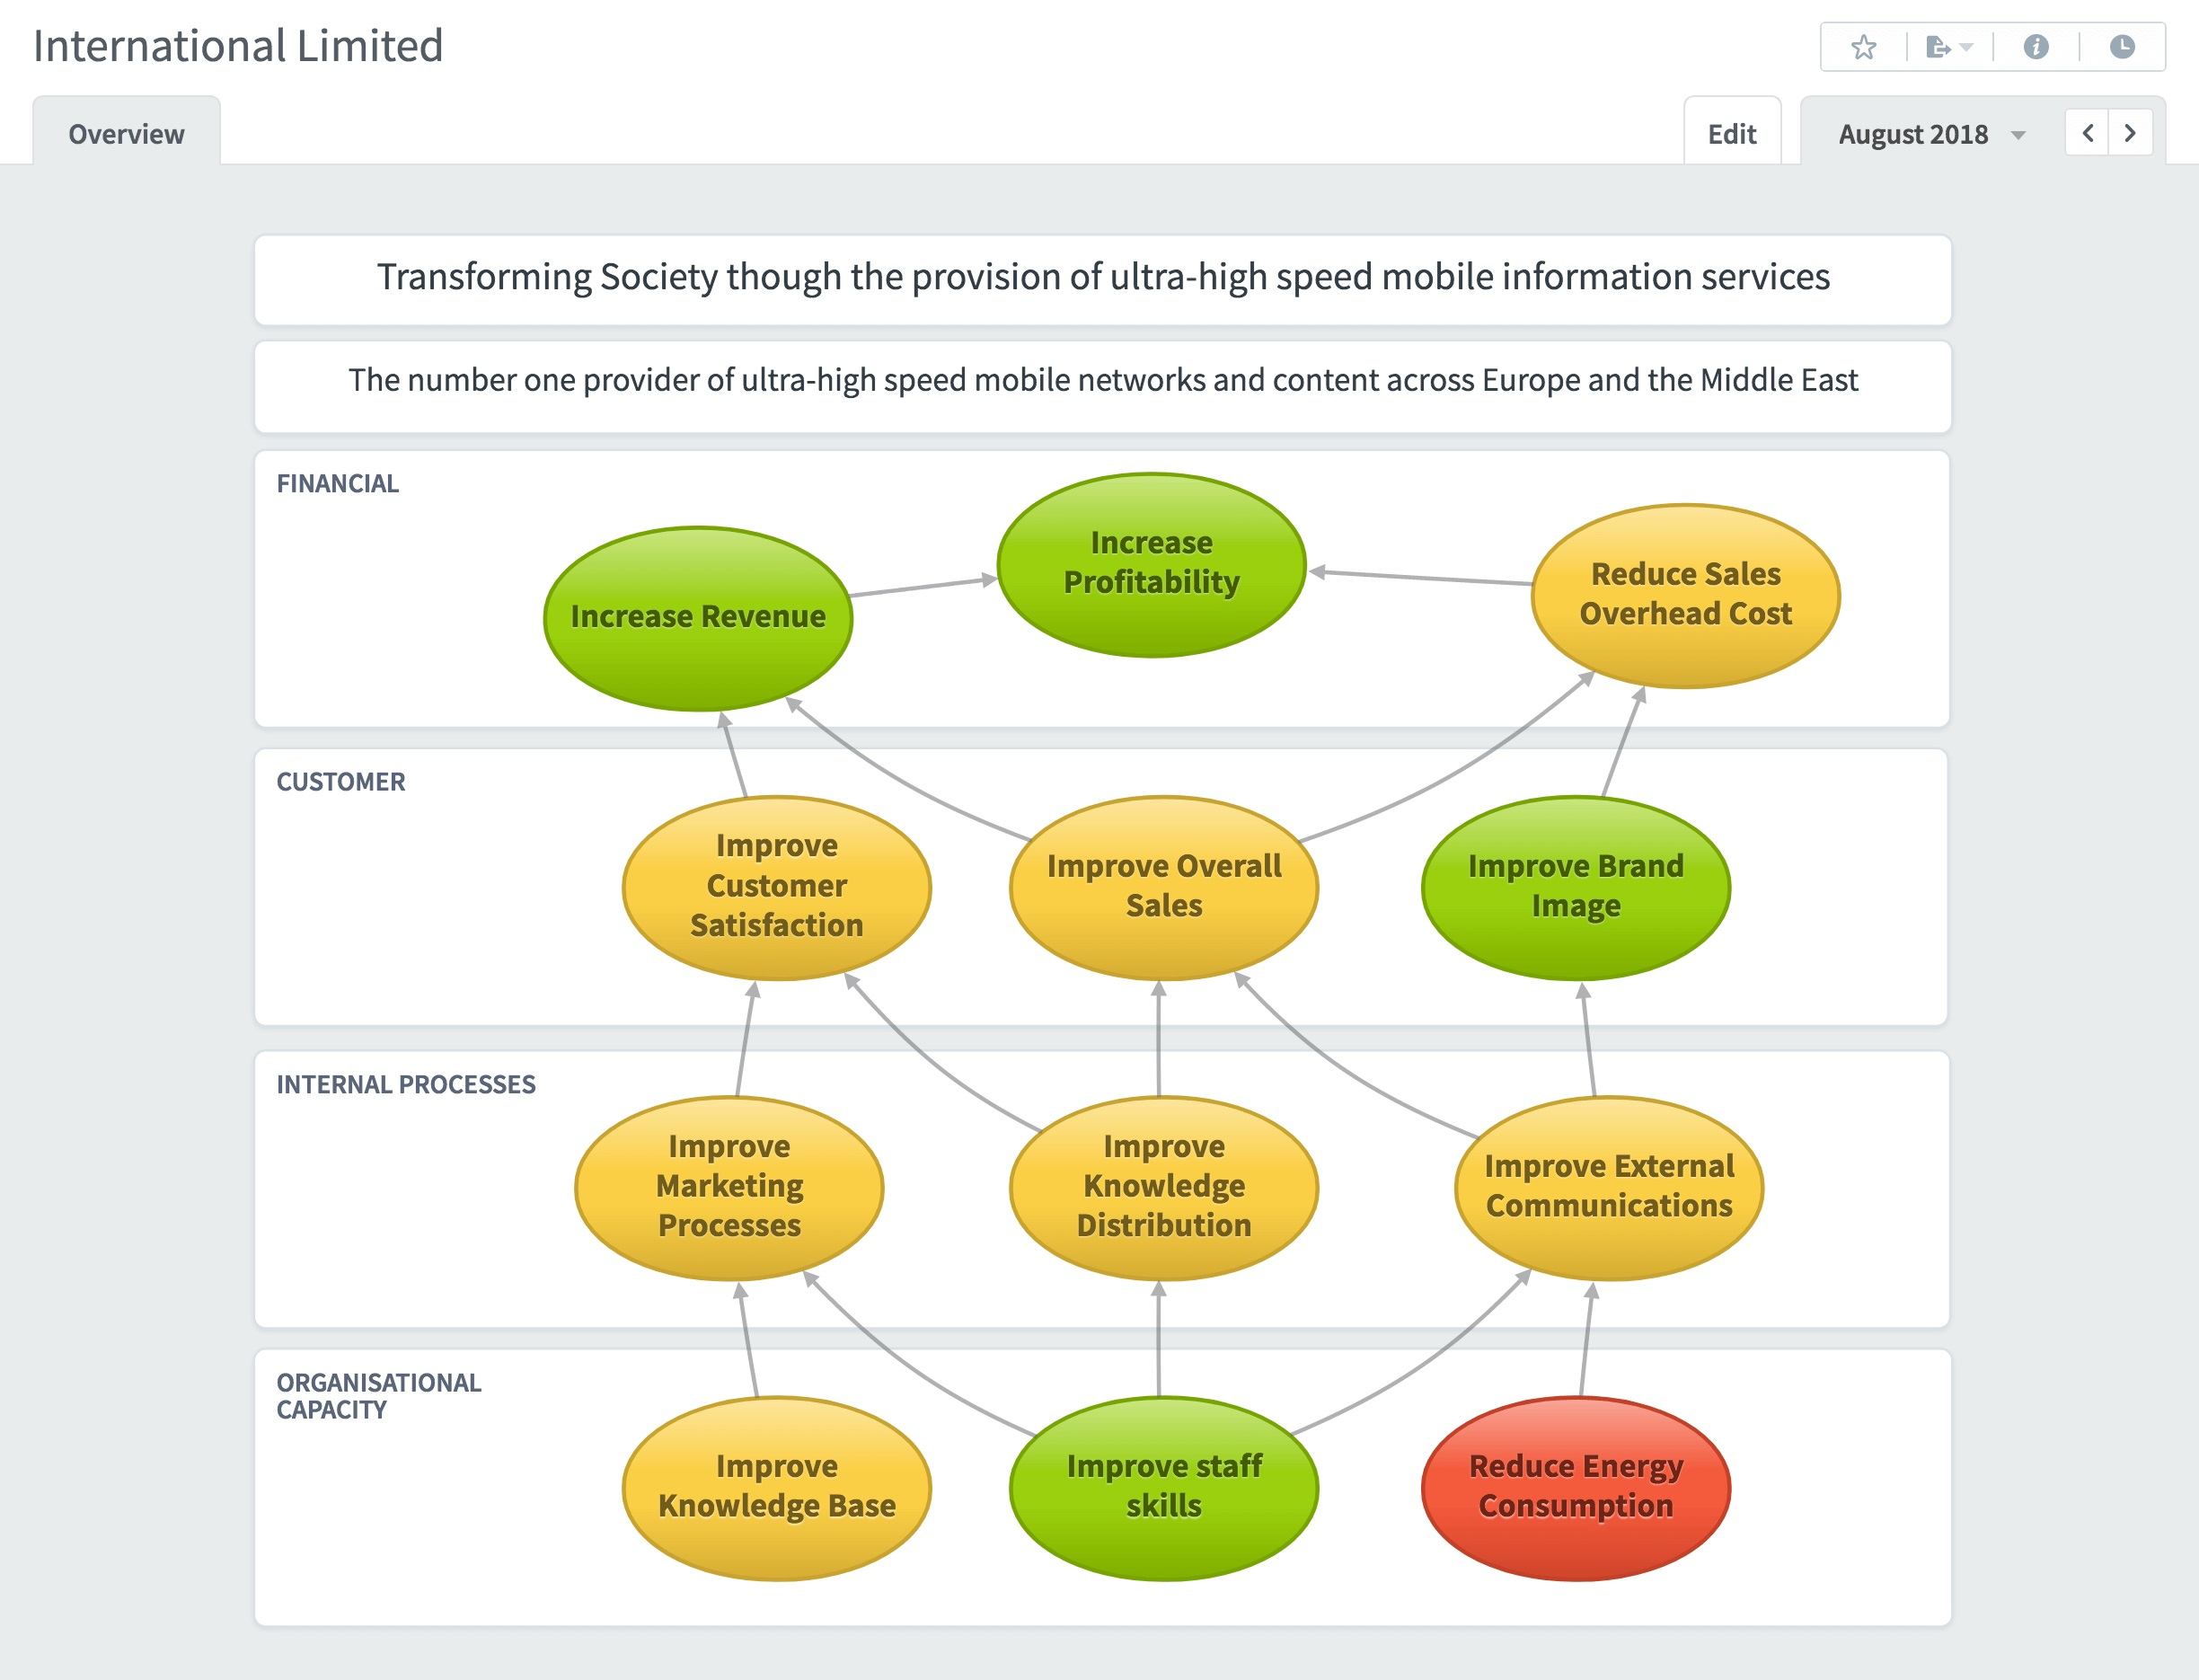
\includegraphics[width=15cm]{./Imagenes/img11}
\end{center}

\section*{¿Cómo funciona el Balanced Scorecard?}
\item{El proceso de creación de un BSC comienza con la determinación de los siguientes parámetros:
\\
\textbf{}
\\
- Objetivos a alcanzar por la organización.\\
- Indicadores o mediciones más adecuados para poder controlar el grado de alance de los objetivos.\\
- Metas concretas en relación a los resultados específicos de dichas mediciones.\\
- Acciones, iniciativas proyectos o programas que se van a implementar para lograr dichas acciones.

\\
\textbf{}
\\
Una vez fijados todos estos factores, el siguiente paso es colocar todas estas mediciones, metas y objetivos en un panel o cuadro, utilizando para ellos un software específico donde se monitorea el progreso de cada uno de ellos.
\\
\textbf{}
\\
Los datos, que normalmente se obtienen de los sistemas informáticos de la empresa, se presentan de manera esquemática y muy gráfica en un panel similar al que utilizan los pilotos de aviones, por lo que también se le conoce como «Cuadro de Mando Integral».}

\section*{Perspectivas del Balanced Scorecard}
\item{A pesar de que son 4 las perspectivas que tradicionalmente identifican un BSC, no es indispensable que estén todas ellas; estas perspectivas son las más comunes y pueden adaptarse a la gran mayoría de las empresas, y no constituyen una condición indispensable para construir un modelo de negocios.}

\begin{center}
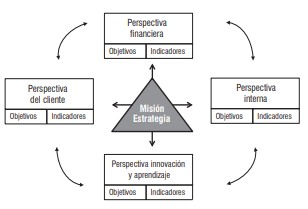
\includegraphics[width=10cm]{./Imagenes/img2}
\end{center}

\item - Perspectiva financiera: ¿cómo debe aparecer la empresa ante sus accionistas/inversores para tener éxito financiero?
\item - Perspectiva del cliente: ¿cómo debe aparecer la empresa ante sus clientes para alcanzar su misión?
\item - Perspectiva interna: ¿en qué debe la empresa ser excelente para satisfacer a accionistas/inversores y clientes?
\item - Perspectiva de innovación y aprendizaje: ¿cómo mantendrá la empresa su capacidad, mejorando y cambiando para conseguir lograr su misión?

\begin{center}
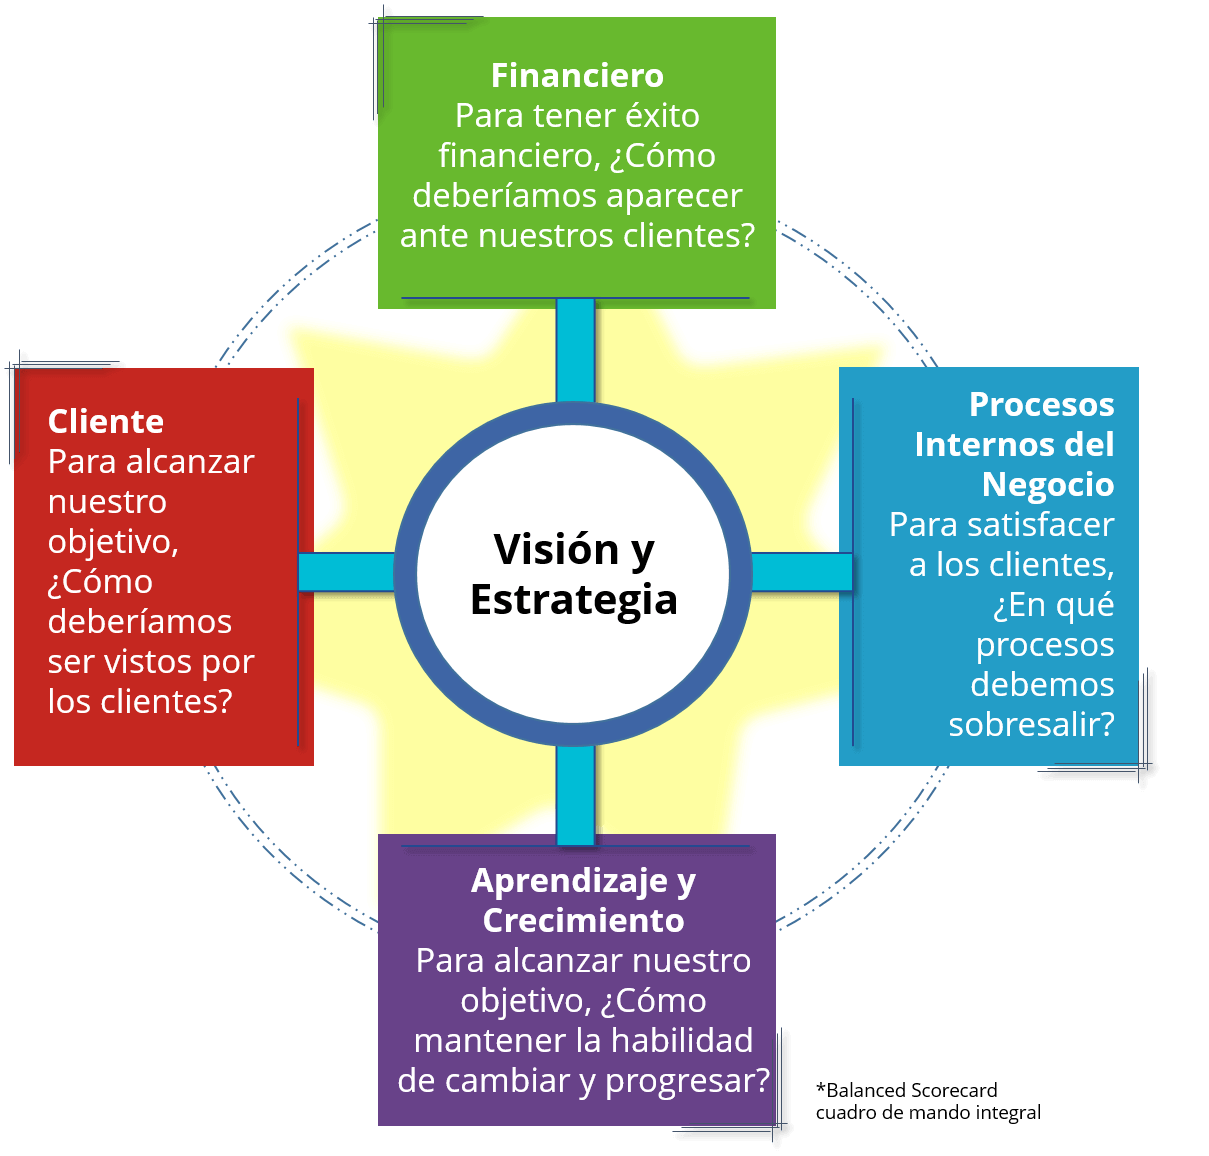
\includegraphics[width=10cm]{./Imagenes/img4}
\end{center}

\section{Beneficios} 
\item{El Balanced Scorecard induce una serie de resultados que favorecen la administración de la compañía, pero para lograrlo es necesario implementar la metodología y la aplicación para monitorear, y analizar los indicadores obtenidos del análisis. Entre otros podemos considerar las siguientes ventajas:}
\\

\item - Alineación de los empleados hacia la visión de la empresa.
\item - Comunicación hacia todo el personal de los objetivos y su cumplimiento.
\item - Redefinición de la estrategia en base a resultados.
\item - Traducción de la visión y estrategias en acción.
\item - Favorece en el presente la creación de valor futuro.
\item - Integración de información de diversas áreas de negocio.
\item - Capacidad de análisis.
\item - Mejoría en los indicadores financieros.
\item - Desarrollo laboral de los promotores del proyecto.

\begin{center}

\includegraphics[width=10cm]{./Imagenes/img5}
\end{center}

\section{Plan Estratégico}
\item{Es un proceso sistemático de desarrollo e implementación de planes para alcanzar metas, propósitos y objetivos.}
\\
\item \textbf{y debe:}
\item - Ser capaz de alcanzar el objetivo deseado
\item - Factible apropiada
\item - Debe proporcionar una ventaja competitiva
\item - Capaz de adaptar a las situaciones cambiantes
\item - Medible en términos de su efectividad

\section{Modelo Canvas}
\item{El modelo canvas es la herramienta para analizar y crear modelos de negocio de forma simplificada. Se visualiza de manera global en un lienzo dividido en los principales aspectos que involucran al negocio y gira entorno a la propuesta de valor que se ofrece.
\\
El modelo canvas se utiliza para pasar de idea a proyecto y plasmar nuestra idea en un modelo empresarial. Es un modelo “vivo”, es decir, que vamos modificando según se va desarrollando, vamos validando clientes, surgen nuevas ideas… por eso se utilizan post-its para completarlo.
}

\section{Generar un modelo canvas}
\item{Muestra de manera lógica la interconexión entre los 9 aspectos básicos de un modelo de negocio. A continuación, mostramos cómo se debe completar un modelo canvas, en qué orden y qué significa cada apartado del lienzo.}
\\
\item \textbf{6.1. Segmento de clientes}
\item{Detectar las necesidades del mercado, del cliente. Nuestro foco siempre es el cliente y debemos orientar el producto a sus necesidades y deseos.\\
Para poder identificar a nuestro cliente debemos ponernos en su piel y analizar qué es lo que piensa, siente, ve, escucha, cuáles son sus problemas y los beneficios que le puede aportar nuestro producto/servicio.\\\\
Debemos dar respuesta a:\\
¿Para quién estamos creando valor?\\
¿Quiénes son nuestros clientes más importantes?}
\\
\item \textbf{6.2. Propuesta de valor}
\item Es la pieza clave de todo el modelo de negocio. La propuesta de valor o ventaja competitiva es el motivo por el que el cliente nos va a comprar a nosotros y no a otro. Aquí se incluye lo que hace diferente e innovador a nuestro producto/servicio.\\
Se puede innovar en diferentes aspectos como en el modelo de ingresos, alianzas empresariales, procesos productivos, entrega del producto/servicio, marca…\\\\
Debemos dar respuesta a:\\
¿Qué valor estamos entregando a nuestros clientes?\\
¿Qué problema resolvemos?\\
¿Cuál es la necesidad que satisfacemos?\\
¿Qué tipo de producto ofrecemos?
\\

\item \textbf{6.3. Canales}
\item Una vez definidos nuestros clientes y la propuesta de valor que les ofrecemos, tenemos que llegar a ellos. Si no nos conocen, no nos van a comprar. Aquí vamos a definir los canales de distribución del producto o servicio.\\\\
Debemos dar respuesta a:\\
¿Con qué canales podemos llegar a nuestros clientes?\\
¿Qué canales funcionan mejor?\\
¿Cuáles de estos canales son los más rentables?
\\
\item \textbf{6.4. Relación con los clientes}
\item Debemos comunicarnos correctamente con nuestros clientes y estar pendiente de ellos. Ellos son nuestro eje central, por lo que saber definir la relación que vamos a tener con cada segmento de clientes, es fundamental para el éxito de un negocio.\\\\
Debemos dar respuesta a:\\
¿Cuál es la relación que tenemos con cada uno de nuestros segmentos de clientes?\\
¿Qué tipo de relación esperan?\\
¿Qué coste tiene?\\\\

\item \textbf{6.5. Flujo de ingresos}\\
\item Para que un negocio sea rentable y podamos sobrevivir en el mercado, tenemos que pensar ¿Cómo monetizarlo? Es decir ¿De dónde vamos a obtener la facturación?\\\\
Debemos dar respuesta a:\\
¿Cuál es nuestra principal línea de ingresos? \\
¿Cómo pagarán nuestros clientes?\\
¿Por qué están dispuestos a pagar nuestros clientes?\\\\

\item \textbf{6.6. Recursos clave}
\item Conocer con qué recursos contamos y con los que debemos contar para llevar a cabo la actividad de nuestro negocio, es clave a la hora de establecer el plan de negocios. Debemos de ser cautos y prudentes a la hora de definir estos recursos. Siempre debemos pensar en la forma de optimizarlos, es decir, intentar conseguir la máxima productividad posible al mínimo coste.\\\\
Debemos dar respuesta a:\\
¿Qué recursos esenciales requiere nuestra propuesta de valor?\\\\

\item \textbf{6.7. Actividades clave}\\
\item Para llevar a cabo la propuesta de valor que queremos ofrecer a nuestros clientes, son necesarias ciertas actividades para preparar el producto antes de que llegue al mercado. Es decir, aquí pensamos en el core de nuestro negocio, lo que haremos en nuestro día a día.\\\\
Debemos dar respuesta a:\\
¿Qué actividad básica requiere nuestra propuesta de valor?\\
¿Cuáles son nuestros canales?\\
¿Cuáles son nuestras fuentes de ingresos?\\\\

\item \textbf{6.8. Aliados clave}\\
\item Para llevar a cabo un negocio, es imprescindible tener aliados. Estos aliados pueden ser;\\\\
Una serie de socios/colaboradores: una buena red de partners nos pueden ayudar a llegar más rápido al cliente, a ir avalados por su reputación y experiencia.\\
Los proveedores: aquellos que nos proporcionan los recursos clave para poder ofrecer los servicios/producto final.\\\\
Debemos dar respuesta a:\\
¿Quiénes son nuestros socios clave en el mercado?\\
¿Quiénes son nuestros proveedores?\\

\item \textbf{6.9. Estructura de costes}\\
\item Obviamente, toda esta infraestructura tiene unos costes que debemos pagar y optimizar. Debemos definir cuáles son nuestras prioridades y los gastos fundamentales en el negocio de aquellos que no lo son.\\
Tener bien clara esta estructura nos ayudará a no desviarnos de los presupuestos y que el negocio fracase por problemas de financiación.\\\\
Debemos dar respuesta a:\\\\
¿Cuáles son los costes más importantes dentro de nuestro modelo de negocio?\\
¿Qué recursos clave son los más costosos?\\
¿Qué actividades clave son las más costosas?\\

\begin{center}
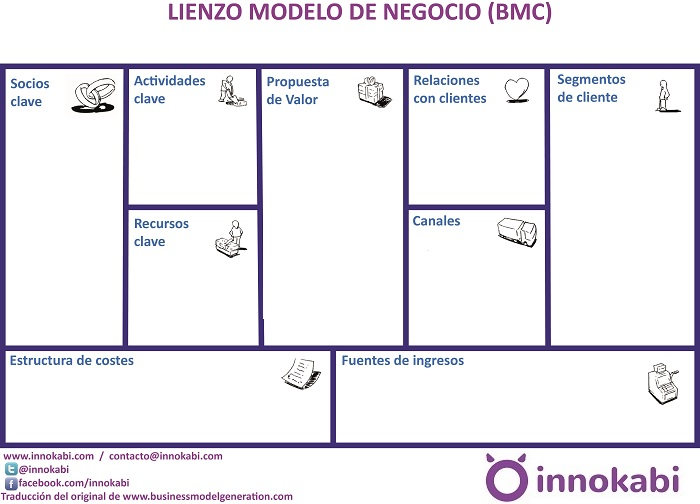
\includegraphics[width=15cm]{./Imagenes/img6}
\end{center}


\section{Ventajas}
\item - Simplicidad de interpretación. la distribucion organizada de los  9 elementos permite dicha simplicidad.
\item - Enfoque integral y sistémico. la interpretación de todos los elementos hace mas visible cualquier posible incoherencia.
\item - Cambios y repercusiones. El analisis de cada alternativa nos permite tantear la viabilidad de cambios.
\item - Cualquier tamaño, cualquier actividad. Es un modelo aplicable a todo tipo de negocio, con independencia de su objeto y de su cifra de negocio.
\item - Sinergia y trabajo en equipo. La simplicidad del método, facilita la generación de ideas y distintos aportes de un grupo de personas que se reúna para desarrollarlo. 
\item - Análisis estratégico en una hoja. Poderosa herramienta para el análisis estratégico: FODA, análisis del mercado, competidores, clientes, proveedores, estructuras y procesos.

\section{Desventajas}
\item - Poco precisa, no sirve para operativa concreta.
\item - Se debe complementar con mapa de procesos detallados.
\item - Por ser tan novedosa puede hacernos creer que completando el lienzo ya tenemos el modelo resuelto


% Bibliografía.
%-----------------------------------------------------------------
\begin{thebibliography}{99}
\item Anzola, P., Bayona, C. & García, T. (2015). "La generación de valor a partir de innovaciones organizativas: efectos directos y moderadores". Universia Business Review, 46: 70-93. 
\item Bastidas, E., Ripoll, V. & Moreno, Z. (2011). "Cuadro de mando multidimensional: propuesta de diseño para la empresa pública de transporte ferroviario de mercancías Renfe-operadora-España". Revista Científica Teorías, Enfoques y Aplicaciones en las Ciencias Sociales, 4(8): 65-78.  
\item Da Silva, J., Pastor, A. & Pastor, J. (2013). "El uso del Cuadro de Mando Integral como instrumento de medición para comparar los modelos de excelencia en gestión". Revista Ibero-Americana de Estratégia, 13(4): 18-3
\item Davila, A. & Oyon, D. (2009). "Introduction to the Special Section on Accounting, Innovation and Entrepreneurship". European Accounting Review, 18(2): 277-280. 


\item https://www.isotools.org/2015/02/23/que-es-el-balanced-scorecard-conoce-su-funcionamiento-y-ventajas/\\
\item https://economipedia.com/definiciones/modelo-canvas.html\\
\item http://www.infoviews.com.mx/Bitam/ScoreCard/]\\
\item https://innokabi.com/canvas-de-modelo-de-negocio/\\
\item https://josefacchin.com/modelo-canvas-de-negocio/\\
\item https://www.adaptiveus.com/balanced-scorecard-vs-business-model-canvas/\\



\end{thebibliography}

